\documentclass[11pt,twoside]{amsart}
\usepackage{/home/alex/.latex/stylesheet}
\usepackage{graphicx}
\usepackage{hyperref}
\usepackage{caption}
\usepackage{subcaption}
\graphicspath{ {./images/} }
\usepackage[backend=bibtex,style=numeric-comp,natbib=true]{biblatex}
\bibliography{paper}


\theoremstyle{theorem}
\newtheorem{theorem}{Theorem}
\newtheorem{corollary}[theorem]{Corollary}
\newtheorem{proposition}[theorem]{Proposition}
\newtheorem{lemma}[theorem]{Lemma}
\theoremstyle{definition}
\newtheorem{definition}[theorem]{Definition}
\newtheorem{example}[theorem]{Example}
\theoremstyle{remark}
\newtheorem{remark}[theorem]{Remark}

\title{Further Investigations into Schelling's Model}
\author{Alex Ledger}
\date{}
\pagestyle{plain}


\begin{document}
\maketitle
\tableofcontents

\newpage

\section{Introduction}
The goal of this paper is two fold. 
First, we wish to find where Schelling's model breaks down; that is, for what parameters does Schelling's model fail to exhibit the expected emergent behavior?
Second, we wish to add to the tools for analyzing the question: to what extent can we make conclusions about reality based on information provided by Schelling's model.
We assume the reader is familiar with the ideas of complex systems, emergent behavior and cellular automata to the extent that one would learn in Mark Bedau's Philosophy of Computation course. 

\section{Review of Schelling's Model}
Schelling's model is a cellular automata presented by Schelling in a 1978 paper \cite{schelling}. 
It is meant to model segregation between groups of people of different interests. 

In the original model, Schelling uses pennies and dimes to represent two classes of people. 
For simplification of the idea, we simply refer to the two classes as white agents and black agents. 
Hence a cell can take on three possible states: it can be empty, be occupied by a white agent, or occupied by a black agent. 
Schelling randomly places black and white agents on a $8 \times 8$ checkerboard. 
Then Schelling stipulates that every white agent wants at least half of their neighbors to be white, and every black agent wants at least a third of their neighbors to be black.
Any agent whose preferences are not met is deemed unhappy. 
For each turn, select one unhappy agent at random and move the agent to the nearest cell such that the agent's preferences are met, i.e. the agent is happy.
Keep on moving agents until all agents are happy (it may be the case that this doesn't happen - we will address this in a second). 
After all of the agents are happy, we look at the organization of the agents on the board. 
What we see is that there are groups of white agents and separate groups of black agents: in a word, there is \emph{segregation}.

% address no equilibrium
In some cases, not all of the agents will become happy and the system will remain in flux. 
Despite this, we still witness segregation on the macro scale. 
For further discussion on the behavior exhibited by Schelling's model, we refer to reader to Schelling's original paper, \cite{schelling}, and a survey of cellular automata \cite{thesis}.

For clarity, we offer a formal definition of neighbors.
\begin{definition}[Neighbors]
    The neighbors of an agent is the set of all agents in the $3 \times 3$ square surrounding the agent, where the agent's cell is in the center of the square. 
    We do not include the agent in the calculation of their neighbors. 
    % add figure here
\end{definition}

\section{My Work}
Our goal in the computational portion of our work was to answer the question: for what parameters does Schelling's model fail to exhibit the expected emergent behavior?
In particular, we explore to what extent the emergent segregation in Schelling's model is dependent on moving an unhappy agent to the nearest cell whereby the agent becomes happy.
We investigate the implications of changing the moving procedure to having the agent go on a random walk and stopping the walk when (a) the agent finds an empty where they would be happy, (b) the agent visits more than $x$ cells at which point the agent returns to their original position and remains unhappy, or (c) the agent visits more than $x$ cells at which point agent settles in the current cell if it is empty (even if they are unhappy) or otherwise returns to their original position.
We call the original model where the agents move to the nearest cell such that they are happy \emph{nearest}, and we call the model where the agents take a random walk \emph{random walk or rw}.

\subsection{What is a random walk?}
Before moving forward, we introduce the notion and implementation of a random walk.
A random walk is, as the name suggests, where an agent moves around the board deciding their path at random. 

The algorithm is quite simple:
\begin{enumerate}
    \item Create set $S$ of all the adjacent cells to the current cell.
    \item Pick a random cell (uniform random) from set $S$.
    \item Move to that cell. 
    \item Repeat the above instructions until the conditions of the agent are met or the number of steps exceeds the alloted amount.
\end{enumerate}

For clarity, if the agent is residing in a cell in the middle of the board, there is a $\frac{1}{4}$ probability that the agent moves in a particular cardinal direction.
If the agent on the board (but not a corner), the agent has a $\frac{1}{3}$ probability of moving to a particular cell of the three adjacent cell.
And if the agent is in a corner, the agent has a $\frac{1}{2}$ probabilty of moving to a particular cell of the two adjance cells.
Importantly, the agent \emph{always} moves; there is a zero probability that the agent stays in the same cell.

It could be the case that in a random walk, the agent moves back and forth between two cells until their $100$ steps are used up - although that is unlikely to occur. 
On the other hand, the agent could walk to every cell on the board, and unfortunately find that no cell makes them happy. 
More likely however, the agent explores some subset of the board at random, and searches for a happy cell.
We did not calculate it, but one certainly could analytically compute the expected number of unique visited cells in a random walk of $100$ steps (assuming the agent does not find a happy cell and end the walk early - that would complicate things).

\subsection{Metrics}
We used two methods for summarazing a state. 
The first is a metric called average similarity. 
We first compute the similarity of each individual agent, this is defined as
\[ \text{similarity(agent)} = \frac{\text{\# neighbors of same race as agent}}{\text{\# neighbors}} \]
Then we compute the average similarity for a state by averaging the similarity of the agents:

\[\text{average similarity(state)} = \frac{\sum_{\text{agent on board}} \text{similarity(agent)}} {\text{\# total agents}} \]
The second metric is called average happiness, is computed:
\[ \text{average happiness(state)} = \frac{\text{\# happy agents}}{\text{\# total agents}} \]
Both average similarity and average happiness are ratios, that is their values are between 0 and 1. 
Moreover, both values, by their nature of being ratios, are largely invariant to the fixed parameters of Schelling's model. 
However, the values do correlate. Since agents in Schelling's model do have a preference to be near agents like themselves, it is expected that as agents become happy, average similarity increases. 

\subsection{Preferences}
The preferences refers the agents' desired compositions of neighbors.
If an agent has a preference ratio of $0.5$, then the agent wants at least half of their neighbors to be of the same race as them.
Alternatively if an agent has a preference ratio of $0.3$, then the agent wants at least $30\%$ of their neighbors to be of the same race as them.
Preferences is the parameters we swept over, in attempt see how the combination of preferences and the moving procedure changed the macro behavior of the system, in the particular the average similarity.
We kept the preferences of the black agents constant at $0.3$ through all of the trials.
We changed the preferences of the white agents. 
The preferences for white people that we tested were $0.3, 0.4, 0.5, 0.6$, and $0.7$. 
The preferences can be understood with the following intuition: as the preference ratio increases, the agent becomes selective about their neighbors, i.e. the agent becomes more racist. 

The preferences are preset before the model begins running; the preferences of agents do not change over time. 


\subsection{Procedure}
We computed a board state randomly using the following algorithm: 
\begin{enumerate}
    \item Initialize the each cell as empty.
    \item For each cell, pick an element of $\{0,1,2,3\}$ uniformly random. If $0$, put a white person in the cell, if $1$ put a black in the cell, and otherwise leave the cell as empty.
        \begin{itemize}
            \item It is worth mentioning that we ran the models with $\{0,1,2\}$ and the results had less elasticicity to the inputted parameters than initializing the board with $\{0,1,2,3\}$. In other words, when the board was less dense (approximately $50\%$ full from $66\%$ full), changes in the parameters had a larger effect on the average similarity and average happiness. 
        \end{itemize}
\end{enumerate}
We ran the nearest model and the random walk model using the same randomly contructed initial state. 
After moving an agent, we recorded the average similarity and average happiness. 
For each set of preferences, we did 25 trials of the nearest simulation and the random walk simulation.

\subsection{Results and Analysis}
As mentioned, we did 25 trials of each model for each set of preferences. 
For each set of 25 trials, we computed the average of the average similarity for each iteration. 
We did likewise for the average happiness. 
The figures are at the end of the document.

Figure \ref{fig:nearest_vs_rw} is the basic result for comparing nearest and random walk.
The random walk is set such that the agents do not return to their original cell if the random walk is unsuccessful. 
There is a more in depth discussion of this setting below. 
The results of \ref{fig:nearest_vs_rw} suggest the nearest model preserves the long-term amount of similarity (segregation) independent of the white agents' neighbor preferences better than the random walk model. 
The value that the average similarity converges to in the random walk model increases (i.e. segregation increases) as the white agents' preference ratio increases (i.e. white agents become more selective).
On the other hand, the value that the average similarity converges to in the nearest model seems constant (i.e. the selectivity of the white agents doesn't affect the amount of segregation).

Figures other than figure \ref{fig:nearest_vs_rw} do not compare the nearest model to the rw model. 
Figure \ref{fig:no_stay_black} and figure \ref{fig:no_stay_white} have the random walk setting such that if an agent has an unsuccessful random walk, the agent returns to their original position. 
These two figures address the difference between changing the length of the random walk for white agents and black agents. 
Figure \ref{fig:no_stay_black} and figure \ref{fig:no_stay_white} and their subplots all look remarkably similar.
This result weakly suggests that the maximum number of steps that agents take in their random walk, in the no stay random walk model, does not have significant effect on the average similarity.

Figure \ref{fig:stay_black} should be compared to \ref{fig:no_stay_black}. In figure \ref{fig:stay_black} at the end of their random walk, and in figure \ref{fig:no_stay_black} the agents do not stay at the end of a random walk - they return to their original position.
The subplots of both figure \ref{fig:stay_black} and \ref{fig:no_stay_black} are remarkably similar. 
This suggests that the nature of the random walk, if agents stay or return at the end, have little effect on segregation. 
It should be noted that for this result, we did not tabulate the number of the agents that exhausted their random walk. 
It is possible that most of the agents found a cell where they would be happy before exhausting their alloted number of steps. 
In this case, it wouldn't matter what the end behavior of the random walk is because it is never relevant. 

Figure \ref{fig:stay_black_decomposed} is another graphical representation of the same model as \ref{fig:stay_black}. 
In figure \ref{fig:stay_black_decomposed}, the average happiness metric is decomposed into the average happiness of whites and the average happiness of blacks.
We see in figure \ref{fig:stay_black_decomposed} that the black agents are on average happier than the white agents indepdently of the number of steps that the black agents can take. 
This is likely simple due to the fact that the whites have a lower neighbor preference, that is a lower threshold for being happy, compared to the whites. 
A good further investigation here would be to set the preferences to the same value, try setting them both to $0.3$ and then both to $0.5$ and see if the maximum number of steps in the random walk then effects happiness. 
In fact, this is just decomposing the happiness of figure \ref{fig:rw_same_prefs}.

In figure \ref{fig:rw_same_prefs}, both white agents and black agents have the same neighbor preferences, ($0.5$), but the races have different maximum random walk lengths. Figure \ref{fig:rw_same_prefs} should be compared to the random walk lines of \ref{fig:nearest_vs_rw}. In figure \ref{fig:nearest_vs_rw}, the agents have different neighbor preferences (black has $0.3$ and white has $0.5$). 
Compared to figure \ref{fig:nearest_vs_rw}, the average similarity in figure \ref{fig:rw_same_prefs} increases more (to $0.80$ compare) as the preferences of the white agents increase. 
This suggests that higher preference ratios (i.e. higher selectivity) leads to greater average similarity (i.e. greater segregation) - an intuitive result.


    \begin{figure}[p]
        \center
        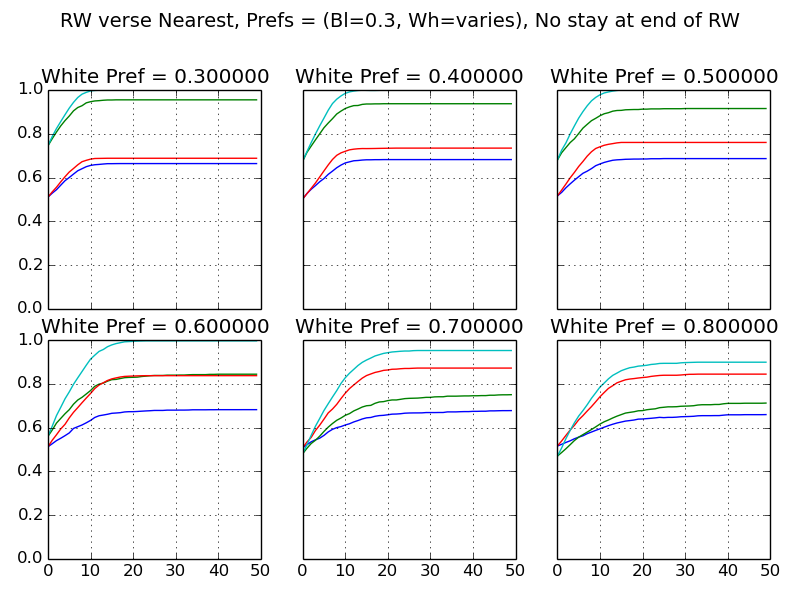
\includegraphics[scale=0.60]{compare_nearest_rw.png}
        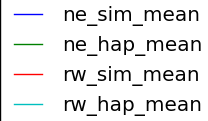
\includegraphics[scale=0.50]{compare_nearest_rw_legend.png}
        \caption{A comparison of random walk verse nearest where the maximum random walk length in 10 steps varied over the preferences of white agents. ``ne'' denotes nearest, ``rw'' denotes random walk, ``sim'' denotes average similarity, and ``hap'' denotes average happiness.}
        \label{fig:nearest_vs_rw}
    \end{figure}

    \begin{figure}[p]
        \center
        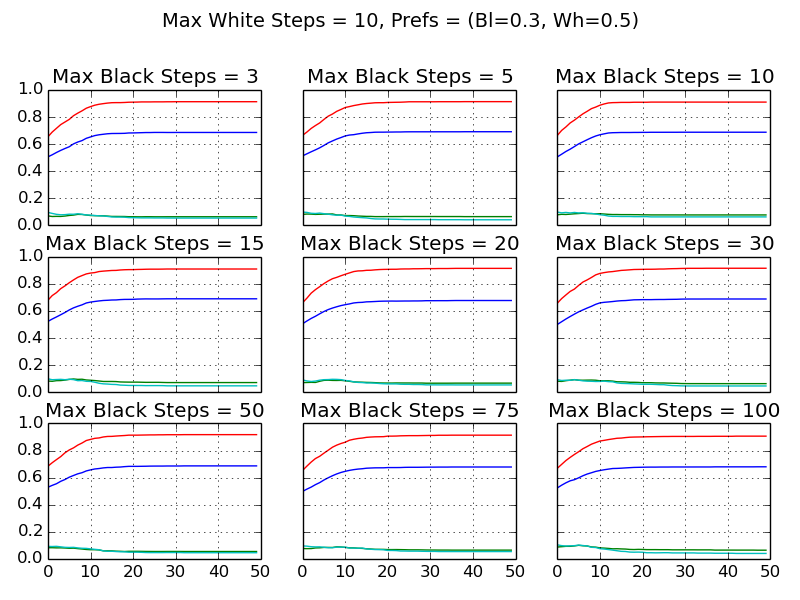
\includegraphics[scale=0.60]{no_stay_at_end_of_rw_change_black_max.png}
        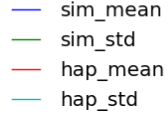
\includegraphics[scale=0.40]{no_stay_at_end_legend.png}
        \caption{Both black and white agents do not stay at the end of a random walk. We vary maximum number of steps that black agents can take during their random walk. White agents prefer greater than or equal to $50\%$ of neighbors to be white, and black agents prefer greater than or equal to $30\%$. }
        \label{fig:no_stay_black}
    \end{figure}

    \begin{figure}[p]
        \center
        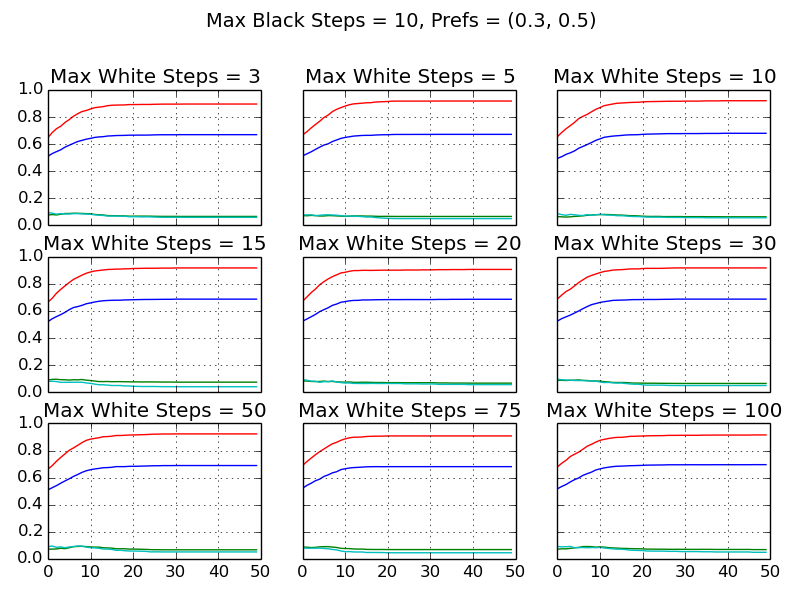
\includegraphics[scale=0.60]{no_stay_at_end_of_rw_change_white_max.png}
        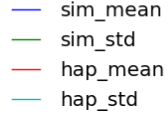
\includegraphics[scale=0.40]{no_stay_at_end_legend.png}
        \caption{Both black and white agents do not stay at the end of a random walk. We vary maximum number of steps that white agents can take during their random walk. White agents prefer greater than or equal to $50\%$ of neighbors to be white, and black agents prefer greater than or equal to $30\%$. }
        \label{fig:no_stay_white}
    \end{figure}

    \begin{figure}[p]
        \center
        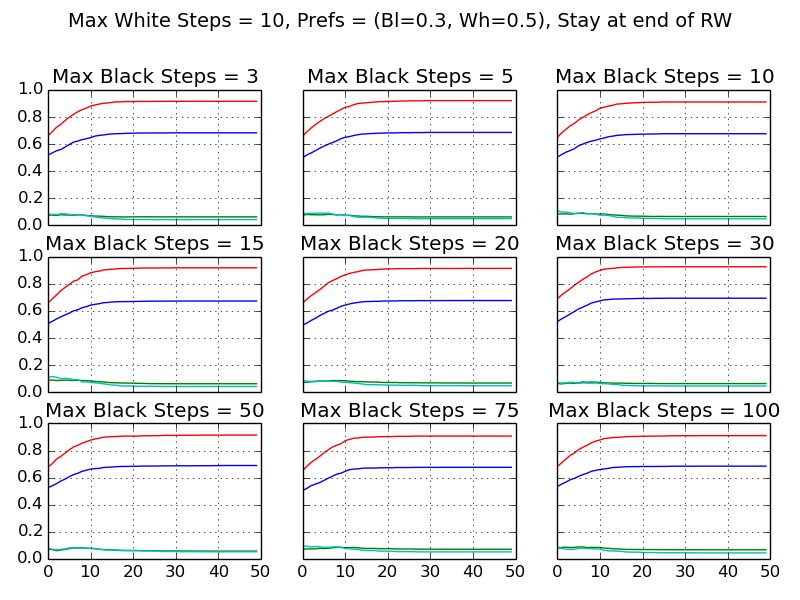
\includegraphics[scale=0.60]{stay_at_end_rw_change_black_max.png}
        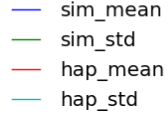
\includegraphics[scale=0.40]{no_stay_at_end_legend.png}
        \caption{Both black and white agents stay at the end of a random walk. We vary maximum number of steps that black agents can take during their random walk. White agents prefer greater than or equal to $50\%$ of neighbors to be white, and black agents prefer greater than or equal to $30\%$. }
        \label{fig:stay_black}
    \end{figure}

    \begin{figure}[p]
        \center
        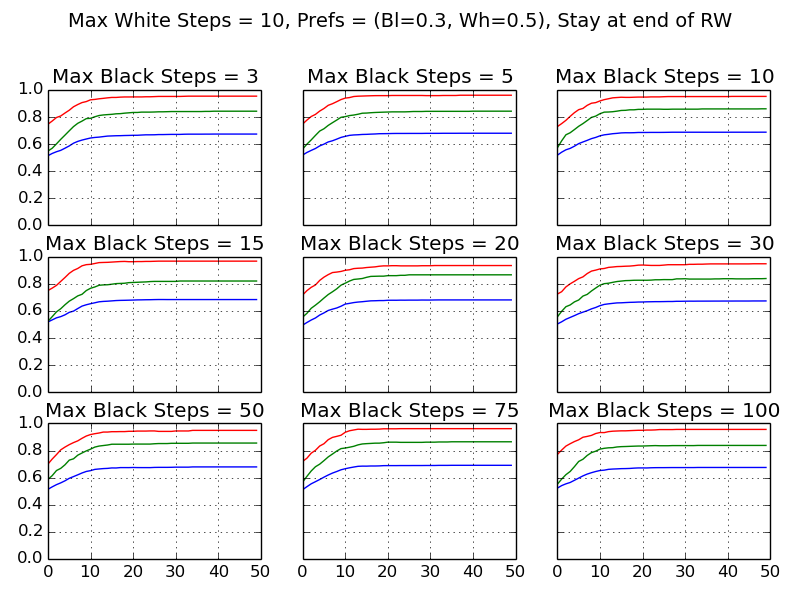
\includegraphics[scale=0.60]{stay_at_end_rw_change_black_max_decompose_happiness.png}
        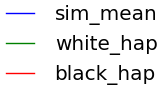
\includegraphics[scale=0.60]{stay_at_end_rw_change_black_max_decompose_happiness_legend.png}
        \caption{Same as figure \ref{fig:stay_black}, but we graph the average happiness of white agents and black agents separately.}
        \label{fig:stay_black_decomposed}
    \end{figure}

    \begin{figure}[p]
        \center
        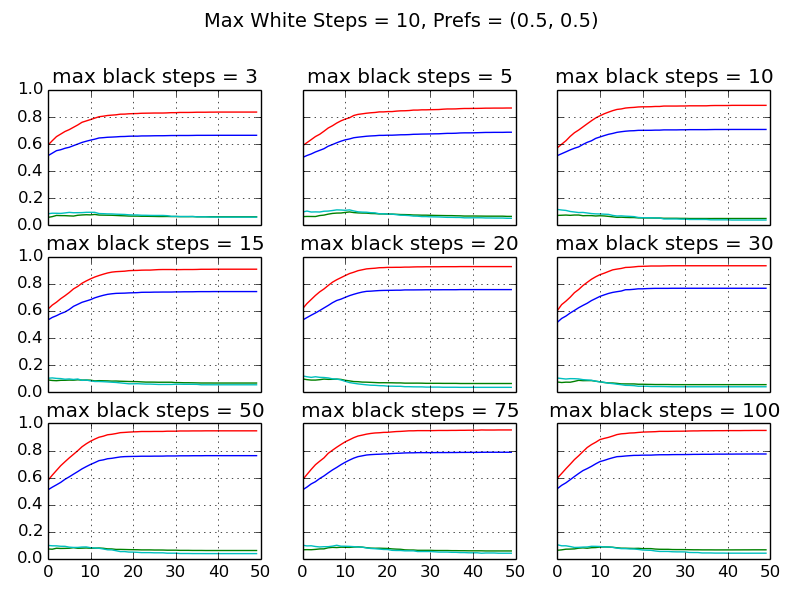
\includegraphics[scale=0.60]{rw_mixed_walk_same_prefs.png}
        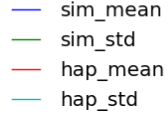
\includegraphics[scale=0.40]{no_stay_at_end_legend.png}
        \caption{Results from the random walk model where black and white agents have the same preferences about their neighbors. Agents do not stay at end of random walk. The changing variable is the amount of steps that black agents can take.}
        \label{fig:rw_same_prefs}
    \end{figure}

\subsection{A list of the parameters in Schelling's model}
    %This definition can be altered by input parameters. Instead of considering the $3 \times 3$ square, we could consider the $x \times x$ square, where $x$ is defined globally.
    \begin{enumerate}
        \item Boundary Conditions
        \item Neighborhood size or vision
        \item Perturb the system: in many biological models, they add random noise to make the model more realistic. 
            Examples of this in Schelling's model are:
            \begin{enumerate}
                \item moving happy agents randomly
                \item Removing and adding agents randomly
                \item Switching the race of a random agent
            \end{enumerate}
        \item Change preferences of models over time based on composition of environment. 
        \item Incoroporate an agent's memory. Maybe someone who lived in mixed race environment for a while will be less racist. And vice versa.
    \end{enumerate}

\section{Conclusion}
Unfortunately given those results, we cannot form any strong conclusions about the nature of schelling's model.
We can however, refine our hypothesis and suggests methods of investigations.

We hypothesize that the core aspect of the Schelling's model is the preference ratios and the fact that agents have a happiness property.
Despite all of the fine tuning and parameter sweeping of parameters related to the movement procedure of agents, Schellng's model never lost its robust segregation: this is particuarly evident in the graphs where standard deviation is plotted. 
Note that the standard deviation is quite low, despite doing 25 trials with random initial configurations. 
Even in data that was not presented in this report, we observed the same robust, low standard deviation when sweeping over paramters affecting the movement procedure. 
We therefore think that the core part of Schelling's model - the part that gives the model its robustness - is the preference ratios and agents being unhappy. 
What is important is that agents are unhappy in some situations, and that unhappy agents do something about their unhappiness; it's less important how the agents do.

In order to investigate this hypothesis, we suggest the following:
\begin{itemize}
    \item Come up with more radical movement procedures and see if the segregation still happens consistently.
    \item Try coming up with slight changes to the preference/happiness parts of Schelling's model. See if segregation still happens consistently.
\end{itemize}

Another intesting investigation that we would be interested in seeing is the reversal of Schelling's model.
Instead of agents only reacting to their environment (i.e. agents being happy/unhappy due to the composition of their neighbors), what if agents were a product of their environment, like certain environments activated and disactivated certain traits of the agents, similar to a biological simulation. 
We suppose that in effect what we are getting at is how can we transform Schelling's model into using traits and evolution?
We are particularly interested in seeing if there would be robust results in the transformation, and more interestingly, if there are robust results, to what extent are they dependent on the preferences/happiness of cell as opposed to the movement procedure, or other auxilliary procedures, involved.
It would be our hypothesis that in such a simulation, the auxilliary procedures would not be the core aspect of the model, just like in Schelling's model.

In conclusion, the core property that Schelling's model robust is property that agents have preferences and that agents do something about their unhappiness, as opposed to the auxilliary procedures such as the movement procedure. 
\printbibliography

\end{document}
